
% Universidad de Costa Rica
% Plantilla para documentación
% Elaborado por Isabel Chaves & Andreína Alvarado
\documentclass[12pt]{article}
\usepackage{vmargin}
\setpapersize{A4}
\setmargins{2.25cm}  % margen izquierdo
{1.5cm}              % margen superior
{16.5cm}             % anchura del texto
{23.42cm}            % altura del texto
{10pt}               % altura de los encabezados
{1cm}                % espacio entre el texto y los encabezados
{0pt}                % altura del pie de página
{2cm}          
\usepackage{blindtext}
\usepackage{listings}
\usepackage[utf8]{inputenc}
\usepackage{lmodern, textcomp}
\usepackage{amsmath}
\usepackage{mathtools}
\usepackage{amsmath}
\usepackage{hhline}
\usepackage{booktabs}
\usepackage{multirow}
\usepackage{colortbl}
\usepackage{color}
\usepackage{xcolor}
\setpapersize{A4}
\usepackage{graphicx}
\usepackage{array}
\definecolor{verdigris}{rgb}{0.26, 0.7, 0.68}
\definecolor{airforceblue}{rgb}{0.36, 0.54, 0.66}
\definecolor{aquamarine}{rgb}{0.5, 1.0, 0.83}
\definecolor{unitednationsblue}{rgb}{0.36, 0.57, 0.9}
\definecolor{pastelblue}{rgb}{0.68, 0.78, 0.81}
\definecolor{turquoise}{rgb}{0.19, 0.84, 0.78}
\definecolor{babyblueeyes}{rgb}{0.63, 0.79, 0.95}
\definecolor{turquoisegreen}{rgb}{0.63, 0.84, 0.71}
\definecolor{uclablue}{rgb}{0.33, 0.41, 0.58}
\definecolor{beaublue}{rgb}{0.74, 0.83, 0.9}
\definecolor{bluegray}{rgb}{0.4, 0.6, 0.8}
\definecolor{cyan(process)}{rgb}{0.0, 0.72, 0.92}
\definecolor{bubbles}{rgb}{0.91, 1.0, 1.0}
\definecolor{mygray}{rgb}{0.4,0.4,0.4}
\definecolor{mygreen}{rgb}{0,0.8,0.6}
\definecolor{myorange}{rgb}{1.0,0.4,0}
\lstset{
basicstyle=\footnotesize\sffamily\color{black},
commentstyle=\color{mygray},
frame=single,
numbers=left,
numbersep=5pt,
numberstyle=\tiny\color{mygray},
keywordstyle=\color{mygreen},
showspaces=false,
showstringspaces=false,
stringstyle=\color{myorange},
tabsize=2,
language=C++,
emph={int,char,double,float,unsigned},
                   emphstyle={\color{blue}}
}
\usepackage{tabu}
\usepackage{amsmath}
%\\usepackage[spanish]{babel}
\graphicspath{{images/}}
\RequirePackage{fancyhdr}
\RequirePackage{fancybox}
\begin{document}
\sffamily


\begin{center}
	\LARGE\textbf{Universidad de Costa Rica}\\
	\textbf{Facultad de Ingeniería}\\
	\textbf{Escuela de Ciencias de la Computación e Informática}\\ \ \\
	\Large 	CI-1310 Sistemas Operativos\\
	Grupo $02|$1\\
	II Semestre
\end{center}


\begin{center}
	\huge\textbf{Tarea programada NachOS\#1}
\end{center}

\begin{center}
	\LARGE\textbf{Profesor:}\\
	Francisco Arroyo\\ \ \\ \ \\
	\LARGE\textbf{Estudiantes:}\\
	Dennis Abarca Quesada $|$ A70014 $|$ grupo 01\\	
	Steven Rojas Lizano 1 $|$ A75623 $|$ grupo 02\\
	
	\textbf{ \today}
\end{center}
\thispagestyle{empty}
\newpage

%--------------------------------------------------------------------------
%----------------------INDICE----------------------------------------------
%--------------------------------------------------------------------------
\tableofcontents

\thispagestyle{empty}
\newpage\setcounter{page}{1}

%--------------------------------------------------------------------------
%----------------------INTRODUCCION----------------------------------------
%--------------------------------------------------------------------------
\newpage
\section[introducción]{Introducción}
En esta tarea programada se realizó la implementación de los llamados al sistema de nachOS, en los cuales se realizaron modificaciones a los archivos de addresSpace, system, exception y machine.\\

%\newpage

%--------------------------------------------------------------------------
%----------------------OBJETIVOS-------------------------------------------
%--------------------------------------------------------------------------

\section[Objetivos]{Objetivos}
\begin{itemize}
  \item    Leer y entender la parte del sistema operativo NachOs que se encuentra en la carpeta descargable.
  \item    Implantar el manejo de excepciones y llamados al sistema. 
  \item    Implantar multiprogramación. 
  \item    Implantar programas de usuario multi-hilos.
\end{itemize}
\section[Descripción]{Descripción}
\begin{enumerate}
  \item Implantar el manejo de excepciones y llamados al sistema. Se deben soportar todos los llamados al sistema definidos en "syscall.h". Presentamos una rutina en ensamblador "syscall" que provee la manera de invocar un llamado al sistema desde una rutina C (Unix tiene un método similar, intente "man syscall"). Usted necesita completar la parte 2 de esta asignación con el fin de probar los llamados al sistema "exec" y "wait"
  \item Implantar multiprogramación. El código que presentamos le restringe a solo poder correr un programa de usuario a la vez. Usted necesita:
   \begin{enumerate}
     \item Encontrar la manera de asignar los marcos de memoria física de tal manera que varios programas de usuario puedan ser colocados en la memoria principal a la vez. (ver "bitmap.h")
     \item Proveer una manera de copiar datos desde/hacia el kernel desde/hacia el espacio de direcciones virtual del usuario (ahora las direcciones que el programa del usuario 've' no son las mismas que el kernel 've')
   \end{enumerate}       
   \item Agregar sincronización a las rutinas que crean e inician el espacio de direcciones, de tal manera que puedan ser accedidas concurrentemente por múltiples programas. Note que "scheduler.cc" ahora guarda y recupera el estado de la máquina en los cambios de contexto. Es deseable tener algunas rutinas como "cp" y "cat" de Unix, y utilizar el shell que proveemos en el directorio "test" para verificar el manejo de llamados al sistema y la multiprogramación
    \item Implantar programas de usuario multi-hilos. Implante los llamados al sistema "fork" y "yield", que le permita al usuario llamar a una rutina en el mismo espacio de direccionamiento, y hacer ping pong entre los hilos (Ayuda: necesita cambiar la manera actual del kernel para asignar memoria en el espacio de direcciones del usuario para cada una de las pilas de los threads)
    \item (Extra, por 5\% )La versión actual del llamado al sistema "exec" no ofrece ninguna manera para que el usuario pueda pasar parámetros o argumentos al nuevo espacio de direcciones creado. Unix permite ésto, por ejemplo, se pueden pasar argumentos en la línea de comandos al nuevo espacio de direcciones. Implantar esta funcionalidad del "exec"
\end{enumerate}

\section[Desarrollo]{Desarrollo}
\subsection{Creación de clases}
Para implementar la solución del problema fue necesario la creación de 3 nuevas clases, las cuales se agregaron a la tarea anterior. 
\subsubsection{Clase Semaphore}
Clase encapsulada del tipo semáforo para mantener el control y la sincronización de los procesos, los métodos utilizados son los mostrados en el libro de referencia y el laboratorio del curso
\subsubsection{Clase Message}
  Al igual que la clase Semaphore, esta clase encapsula el envío y la recepción de los mensajes, además se le agregaron los siguientes métodos:
  \begin{itemize}
    \item \emph{SendMap}: Método que recibe un mapa de string,int y envía mensajes iterando por dicho mapa hasta que este se acabe.
    \item \emph{ReceiveMap}:Método que recibe como parámetro la dirección de un mapa donde guarda todos los mensajes de todos los tipos que se encuentren en la clase reservedWords. Este método leerá mensajes del mismo tipo hasta que de error del tipo NOMSG, al darse este error sigue con el siguiente tipo de palabra reservada.
  \end{itemize}
  \subsubsection{clase ReservedWords}
    Esta es una clase que contiene un mapa que encapsula todas las palabras reservadas, por lo cual es utilizado para la lectura de los archivos, el envío de mensajes y la recepción de los mismos.
    
\subsection[Actualización de Clases]{Actualización de clases}
para agregar la funcionalidad deseada fue necesario actualizar las 2 clases propuestas en la tarea 0, esto se muestra a continuación.
\subsubsection{Clase FileReader}
Se agregó el método GetreservedCount el cual busca en el archivo todas las palabras reservadas y las va guardando en un mapa string int el cual devolverá.

\subsubsection{Clase FileComparator}
Para esta clase se agregó un método igual al de fileReader el cual se encarga de pasar a un nivel superior los mapas encontrados por los archivos

\section{Pruebas}
  Para validar la implementación llevado a cabo, se probará  el sistema operativo con los archivos de prueba create1.c, fork4.c y pingpong.c los cuales son archivos de prueba disponibles en la página web del curso de laboratorio del curso. 
  \subsection{Archivo prueba create1.c}
    \begin{lstlisting}
int main(){
	int fd;
	int e;
        char * buf;
	Create("archivo.nuevo");
	fd = Open("archivo.nuevo");
	Write("prueba", 6, fd) ;
	Close(fd);
//	Exec("../test/rillo");	
	Exec("prueba Exec");

	//char* buf = new int[6];
	fd = Open("archivo.nuevo");
	Read(buf, 6, fd);
	Write(buf, 6, 1);

	Halt();
	return 0;
}      
    \end{lstlisting}
En este caso se prueba los system calls Create, Open, Write, Close, Read y Exec. Como se puede ver en la Ilustración, se ingresa con éxito a los system calls Create, Open y Close. Una vez abierto y cerrado el archivo, envía un mensaje indicando que el archivo se cerró con éxito.
Al ingresar a Exec, muestra que el archivo no se pudo ejecutar dado que no existe. Posteriormente vuelve a abrir el archivo con el SC Open y lee la cantidad de bytes solicitados. En la imagen se muestra que efectivamente esto ocurre.
    \begin{figure}[hbt]
      \begin{center}
        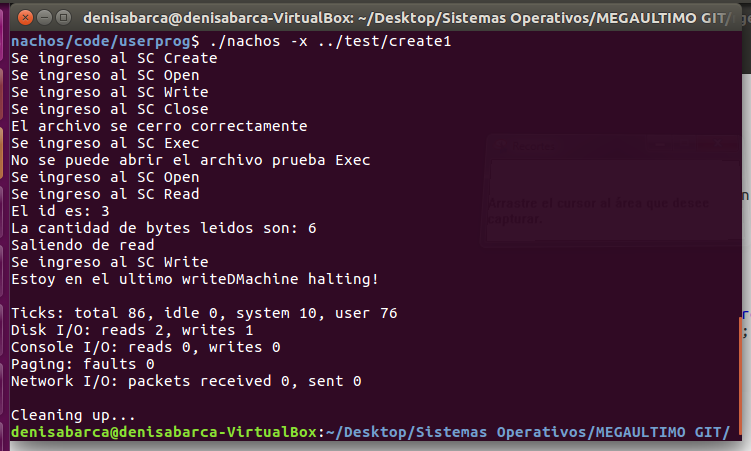
\includegraphics[width=0.5\textwidth]{Prueba_create.PNG}
        \caption{Prueba de create.C}
        \label{fig:create}
      \end{center}
    \end{figure}
\subsection{Archivo prueba: fork4.c}
\begin{lstlisting}
  #include "syscall.h"

void nada(void);
void todo(void);

int semaforoID;

int main(){
	semaforoID = SemCreate(0);
	Fork(nada);
}


void nada(){
	Fork(todo);
	Write("Nada!", 5, 1);
	SemSignal(semaforoID);
}

void todo(){
	Write("Vamos", 5, 1);
	SemWait(semaforoID);
	Write("Final", 5, 1);
}
\end{lstlisting}
En este caso, se prueba el system Call Fork y los system calls asociados a la funcionalidad de los semáforos, es decir; semCreate, semDestroy, semSignal, semCreate. \\
Al inicio, se ingresa con éxito al SC semCreate e inicializa el semáforo en cero. Posteriormente se invoca el System Call Fork. Al crear el Fork la dirección de referencia ejecuta el método void Nada(), en donde al mismo tiempo vuelve a ejecutar el llamado al sistema Fork  ejecutando el método void todo(). \\
En ambos métodos, Vamos y Todo debería ejecutarse los métodos Write mostrando en pantalla los strings ‘Vamos’ y ‘Nada’. Sin embargo, esta prueba presentó el error de que no mostró en pantalla la palabra ‘Nada’ pero sí ‘Vamos’ de los llamados al sistema Write. Lo anterior puede deberse a una falla en la sincronización entre el proceso padre y el proceso hijo.
    \begin{figure}[hbt]
      \begin{center}
        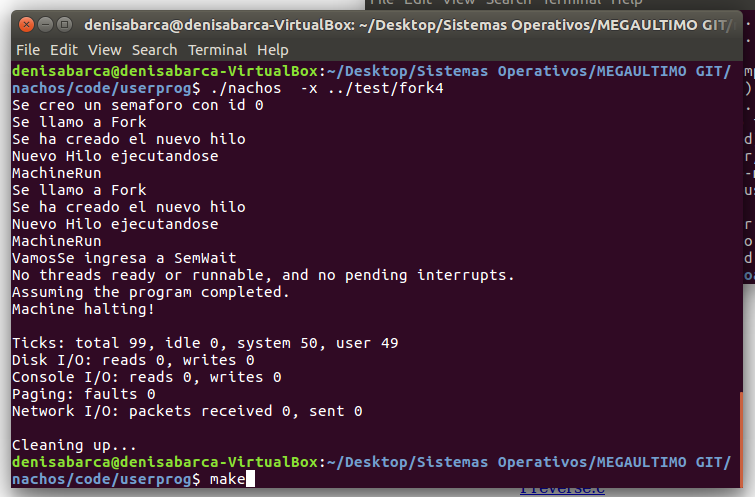
\includegraphics[width=0.5\textwidth]{Prueba_Fork.PNG}
        \caption{Prueba de Fork.C}
        \label{fig:Fork}
      \end{center}
    \end{figure}
    \subsection{Prueba pingPong.c}
    \begin{lstlisting}
#include "syscall.h"

void SimpleThread(int);

int
main( int argc, char * argv[] ) {

    Fork(SimpleThread);
    SimpleThread(1);

    Write("Main  \n", 7, 1);
}

void SimpleThread(int num)
{

    if (num == 1) {
	for (num = 0; num < 5; num++) {
		Write("Hola 1\n", 7, 1);
		Yield();
	}
    }

    else {
	for (num = 0; num < 5; num++) {
		Write("Hola 2\n", 7, 1);
		Yield();
	}
    }
    Write("Fin de\n", 7, 1);
}
\end{lstlisting}
En este caso se analiza la funcionalidad de los métodos Fork y Yield. Consiste en crear un nuevo proceso y posteriormente alternar el hilo que está corriendo empleando el llamado al sistema Yield. \\
Lo primero que ocurre es la creación de un nuevo hilo mediante Fork y posteriormente se llamara al método SimpleThread.\\
Como ahora hay dos procesos e ingresarán a SimpleThread() uno con un valor de argumento igual a 1 y el otro distinto de 1, el llamado al sistema Yield() intercambiará los procesos de manera alternada hasta que se cumple el condicional en el ciclo for. En la Imagen adjunta se muestra que efectivamente esto se logra, ya que Hola 2 y Hola 1 cambian de manera alternada. 
 \begin{figure}[hbt]
      \begin{center}
        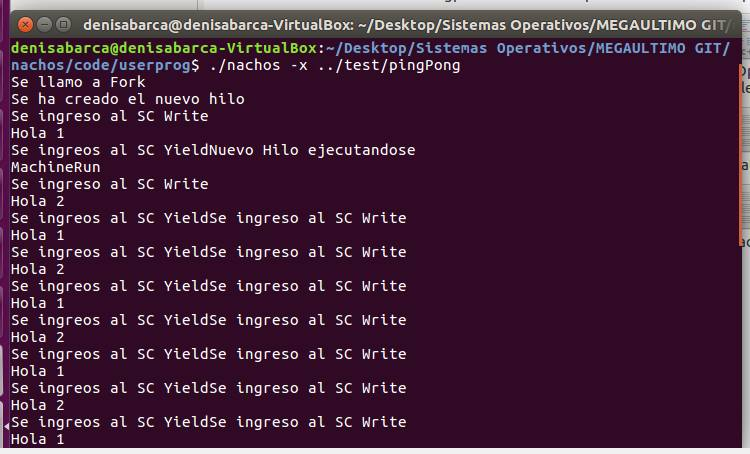
\includegraphics[width=0.5\textwidth]{Prueba_PingPong.PNG}
        \caption{Prueba de Ping Pong.C}
        \label{fig:Fork}
      \end{center}
    \end{figure}

 




%--------------------------------------------------------------------------
%----------------------MANUAL-------------------------------------------
%--------------------------------------------------------------------------
\newpage
\section[Manual de usuario]{Manual de usuario}
\subsection{Requerimientos}
El sistema posee los siguientes requerimientos para su correcto funcionamiento
\begin{itemize}
  \item Sistema operativo Fedora o Ubuntu
  \item Arquitectura 64 bits
  \item Ambiente NachOS 
  \item Compilador: GNU GCC compiler
\end{itemize}

\subsection[Restricciones]{Restricciones del programa}
\begin{itemize}
  \item El sistema solamente puede ser ejecutado desde la terminal.
  \item El sistema solamente trabaja con archivos codificados en UTF-8 y codigos fuente del lenguaje C. 
  \item El simulador MIPS se basa en un único procesador.
  \item el máximo número de páginas es de 32 y cada una es de 128 bytes por lo que los programas de usuario no deben ser mayores a 4kB
  \item EL número máximo de hilos a guardar en la cola es de 20 hilos
  \end{itemize}
\newpage


\section{Bibliografía}

[1] Silberchatz, Abraham, Galvin, Peter \& Gagne, Greg. {\em  Operating Systems Concepts.} Novena edición, Addison Wesley Publishing Co., Mass., 2013 
\end{document}
